%%%%%%%%%%%%%%%%%%%%%%%%%%%%%%%%%%%%%%%%%%%%%%%%%%%%%%%%%%%%%%%%%%%%%%%%%%%%%%%%
%2345678901234567890123456789012345678901234567890123456789012345678901234567890
%        1         2         3         4         5         6         7         8
\documentclass[letterpaper, 10 pt, conference]{ieeeconf}  % Comment this line out
% if you need a4paper
%\documentclass[a4paper, 10pt, conference]{ieeeconf}      % Use this line for a4

\usepackage{float}
% paper
% uso paquete bookmark para tener bien los outlines.
\usepackage{bookmark}

% Configuro el idioma.
\usepackage[utf8]{inputenc} % Importante para mantener acentos.
\usepackage[spanish, activeacute]{babel} % Requiere: texlive-lang-spanish. Por primera vez hay que ejecutar: texconfig init> log

% Paquete para poder usar acentos en $$.
\usepackage{mathtools}
%\setmathfont{XITS math}

\usepackage{tikz}
\usetikzlibrary{shapes.misc, positioning, shapes.geometric, arrows.meta}

\usepackage{siunitx}

% package to get \url
\usepackage{hyperref}
\hypersetup{
  colorlinks=true,
  linkcolor=magenta,
  filecolor=magenta,
  citecolor=magenta,      
  urlcolor=magenta,
}

% Graficos electrónicos
\usepackage{circuitikz}

\IEEEoverridecommandlockouts                              % This command is only
% needed if you want to
% use the \thanks command
\overrideIEEEmargins
% See the \addtolength command later in the file to balance the column lengths
% on the last page of the document

\usepackage{graphicx}
\usepackage{graphics}

% styling for matlab/octave code.
\usepackage{matlab-prettifier}
% Configuracion, con esto puede agregar ñ.
\lstset{
  literate={ñ}{{\~n}}1
}

% The following packages can be found on http:\\www.ctan.org
%\usepackage{graphics} % for pdf, bitmapped graphics files
%\usepackage{epsfig} % for postscript graphics files
%\usepackage{mathptmx} % assumes new font selection scheme installed
%\usepackage{times} % assumes new font selection scheme installed
\usepackage{amsmath} % assumes amsmath package installed
%\usepackage{amssymb}  % assumes amsmath package installed

\title{\LARGE \bf Laboratorio N° 3}

\author{
  Tom\'as Vidal\\
  {\it Circuitos Electrónicos 1}\\
  {\it Facultad de Ingenier\'ia, UNLP, La Plata, Argentina.}\\
  {\it 29 de Junio, 2024.}
}                                            % <-this % stops a space


% comienzo

% INTRO

% Figura
\newcommand{\image}[2] {
  \begin{figure}[H]
    \centering
    \includegraphics[width=0.43\textwidth]{./#1.png}
    \caption{#2}
    \label{fig:#1}
  \end{figure}
}

% Codigo
% \begin{lstlisting}[style=Matlab-editor]
% % el código va aca
% dispc("HELLO WORLD");
% \end{lstlisting}

\begin{document}
\maketitle
\thispagestyle{empty}
\pagestyle{empty}

% \section{INTRODUCCCI\'ON}
% TODO

\section{Topología presentada}
\begin{figure}[H]
 \centering
 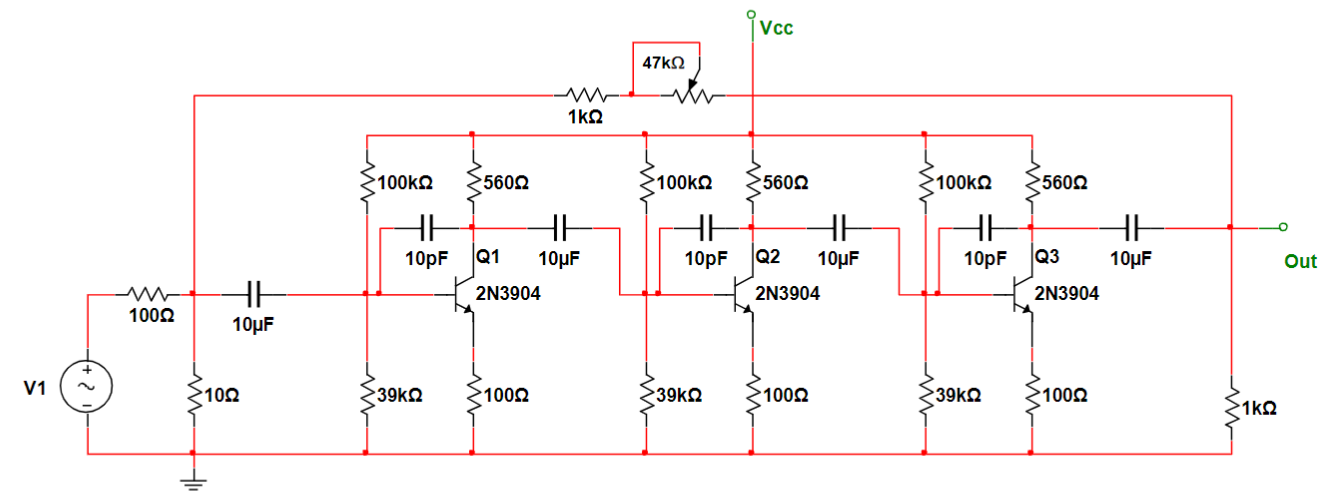
\includegraphics[width=0.43\textwidth]{./Imagenes/circuito_completo.png}
 \caption{Circuito dado}
 \label{pic:circuito_completo}
\end{figure}
\subsection{Circuito completo}
A partir del circuito dado (\ref{pic:circuito_completo}) se pueden identificar 3 etapas individuales de amplificación y una realimentación de las mismas. Por lo que a continuación se analizan estas etapas individuales y el lazo de realimentación
\section{Etapa aislada}
\begin{figure}[H]
  \centering
  \begin{circuitikz}
    \node[npn] (npn) at (0,0) {};
    \draw (npn.base) -- ++(-1, 0) -- ++(0, -1) to[R=$\qty{39}{\kilo\ohm}$] ++(0, -1.5) -- ++(0, -0.5) node[ground]{};
    \draw (npn.base) -- ++(-1, 0) -- ++(0, 1.5) to[R=$\qty{100}{\kilo\ohm}$] ++(0, 1.5) -- ++(0, 0.5) node[ocirc]{} coordinate (Vp) node[right, font=\large] {$+V$}; 
    \draw (npn.collector) -- ++(0, 0.75) to[R=$\qty{560}{\ohm}$] ++(0, 1.5) -- ++(0, 0.5) node[ocirc]{} coordinate (Vp) node[right, font=\large] {$+V$};
    \draw (npn.collector) -- ++(0, 0.5) node[circ]{} -- ++(-0.75, 0) to[C=$\qty{10}{\pico\farad}$] ++(-0.5, 0) -- ++(-0.6, 0) node[circ]{};
    \draw (npn.collector) node[circ]{} -- ++(1, 0) to[C=$\qty{10}{\micro\farad}$] ++(1, 0) -- ++(0.75, 0) node[ocirc]{} coordinate (Vin) node[right, font=\large] {$V_{s}$};
    \draw (npn.emitter) -- ++(0, -0.25) to[R=$\qty{100}{\ohm}$] ++(0, -1.5) -- ++(0, -0.5) node[ground]{};
    \draw (npn.base) -- ++(-1, 0) node[circ]{} -- ++(-1, 0) to[C=$\qty{10}{\micro\farad}$] ++(-1, 0) -- ++(-0.75, 0) node[ocirc]{} coordinate (Vin) node[left, font=\large] {$V_{e}$};
  \end{circuitikz}
  \caption{Etapa individual dentro del lazo directo}
  \label{circ:etapa_individual}
\end{figure}
Este amplificador es uno de \textit{transadmitancia} ($\left[ \frac{A}{V} \right]$), y sus parámetros más representativos para este análisis son los de la tabla \ref{tab:mod_transadmitancia}; los mismos se obtuvieron aplicando el modelo de pequeña señal del BJT, y considerando que el capacitor de $\qty{10}{\pico\farad}$ está en circuito abierto y, los de $\qty{10}{\micro\farad}$ están en cortocircuito en pequeña señal.
\\
\textit{Para calcular la ganancia total de las tres etapas en cascada, se consideró que la última contenía la carga (de \qty{1}{\kilo\ohm}) del circuito}

\begin{table}[H]
  \centering
  \scalebox{0.85}{
    \begin{tabular}{|l|l|l|}
      \hline
                                                & Analítico                                                                                 &  Aproximado       \\ \hline
      $Z_{in}$                                  & $(\qty{100}{\kilo\ohm} // \qty{39}{\kilo\ohm}) // (\qty{100}{\ohm}(1+h_{fe}))$            & \qty{13.2}{\kilo\ohm}  \\ \hline
      $Z_{out}$                                 & \qty{560}{\ohm}                                                                           & \qty{560}{\ohm}   \\ \hline
      $A_{v}$                                   & $\frac{-\qty{560}{\ohm}}{\qty{100}{\ohm}}$                                           &  -5.6                  \\ \hline
      $A_{v}$ (con \qty{1}{\kilo\ohm})  & $\frac{-(\qty{560}{\ohm} // \qty{1}{\kilo\ohm})}{\qty{100}{\ohm}}$                   &  -3.59                         \\ \hline
    \end{tabular}
  }
  \caption{Parámetros del amplificador de transadmitancia}
  \label{tab:mod_transadmitancia}
\end{table}

\section{Lazo directo y realimentación}
Para poder obtener la ganancia de lazo cerrado total del circuito, primero se considera el modelo con un bloque de ganancia de lazo directo \textbf{a} y una de realimentación \textbf{$\beta$} conectados en paralelo, tal como se puede identificar en el circuito completo \ref{pic:circuito_completo}.
\begin{figure}[H]
  \centering
  \begin{circuitikz}

    % bloque de lazo directo
    \node (square) [draw,minimum width=2cm,minimum height=2cm,anchor=south west] at (0,0) {a};
    \draw (square.west) |- ++(-2, 0.5) node[ocirc]{};
    \draw (square.west) |- ++(-2, -0.5) node[ocirc]{};
    \draw (square.east) |- ++(2, 0.5) node[ocirc]{};
    \draw (square.east) |- ++(2, -0.5) node[ocirc]{};

    % bloque de realimentación
    \node (square_b) [draw,minimum width=1.5cm,minimum height=1.5cm,anchor=south west] at (0.25, -2) {$\beta$};
    \draw (square_b.west) |- ++(-0.75, 0.5) -- ++(0, 2.25) node[circ]{};
    \draw (square_b.west) |- ++(-1.25, -0.5) -- ++(0, 2.25) node[circ]{};
    \draw (square_b.east) |- ++(0.75, 0.5) -- ++(0, 2.25) node[circ]{};
    \draw (square_b.east) |- ++(1.25, -0.5) -- ++(0, 2.25) node[circ]{};

  \end{circuitikz}
  \caption{Circuito completo realimentado (transimpedancia)}
  \label{diag:transimpedancia}
\end{figure}

La ganancia de lazo directo \textbf{a} corresponde a las tres etapas en cascada considerando la última cargada con la resistencia de \qty{1}{\kilo\ohm}. La del bloque beta corresponde a la que se obtiene al aplicar los parámetros \textbf{Y} (en el bloque de realimentación \ref{diag:bloque_beta}). Estos valores se pueden observar en la tabla \ref{tab:ganancias_de_a_y_beta}. \textit{Posteriormente se refiere a la resistencia de la red de realimentación como $R_{f}$, de feedback, esta es la resistencia de \qty{1}{\kilo\ohm} en serie con el potenciómetro}

\begin{figure}[H]
  \centering
  \begin{circuitikz}

    % bloque de lazo directo
    \node (square) [draw,minimum width=4cm,minimum height=3.5cm,anchor=south west] at (0,0) {$\beta$};
    \draw (square.west) ++(-1, 0.75) node[ocirc]{} -- ++(1.5, 0) to[R=\qty{1}{\kilo\ohm}] ++(1.25, 0) to[vR=\qty{47}{\kilo\ohm}] ++(2,0) -- ++(1,0) -- ++(0.25,0) node[ocirc]{};
    \draw (square.west) ++(-1, -0.75) node[ocirc]{} -- ++(6,0) node[ocirc]{};

  \end{circuitikz}
  \caption{Bloque beta de realimentación}
  \label{diag:bloque_beta}
\end{figure}

\begin{table}[H]
  \centering
  \begin{tabular}{|l|l|l|l|}
    \hline
    Admitancias terminales                  & Analítico                       & $R_f=\qty{48}{\kilo\ohm}$  & $R_f=\qty{1}{\kilo\ohm}$            \\
    \hline
    De entrada $y_{11}$ & $\frac{1}{R_f}$   & \qty{20.8}{\micro\siemens}      & \qty{1}{\milli\siemens}                          \\
    \hline
    De salida $y_{22}$ & $\frac{1}{R_f}$    & \qty{20.8}{\micro\siemens}      & \qty{1}{\milli\siemens}                          \\
    \hline
  \end{tabular}
  \caption{Parámetros de la realimentación}
  \label{tab:param_bloque_beta}
\end{table}

\begin{table}[H]
  \centering
  \scalebox{0.85}{
    \begin{tabular}{|l|l|l|}
      \hline
      Ganancia & Analítico & Aproximado \\
      \hline
      $a_v$ & $(A_v)(A_v)(A_{v cargado})$ & $(-5.6)(-5.6)(-3.39) \cong -112.6 \left[ \frac{V}{V} \right]$  \\
      \hline
      $ \beta_{max}$ & $ \frac{-1}{\qty{1}{\kilo\ohm}}$ & $ -1m \left[ \frac{A}{V} \right] $ \\
      \hline
      $ \beta_{min}$ & $\frac{-1}{\qty{48}{\kilo\ohm}}$ & $-20\mu \left[ \frac{A}{V} \right] $ \\
      \hline
    \end{tabular}
  }
  \caption{Ganancia de los bloques}
  \label{tab:ganancias_de_a_y_beta}
\end{table}

\textit{El potenciómetro que ajusta la realimentación hace que la ganancia $\beta$ ($\beta_{max}$) sea máxima, cuando el potenciómetro está al mínimo (es decir \qty{0}{\ohm}), y de manera análoga, cuando el potenciómetro se encuentra la máximo (\qty{48}{\kilo\ohm}) la ganancia $\beta$ es mínima ($\beta_{min}$)}

\subsection{Ganancia de transimpedancia}
Hasta ahora la ganancia del lazo directo calculada es de tensión (tabla \ref{tab:ganancias_de_a_y_beta}), pero para hacer la realimentación del circuito completo se debe considerar una ganancia de transimpedancia a lazo abierto (\ref{eq:ganancia_de_transimpedancia_la}). \textit{Para obtenerla se aplicó la ley de Ohm en la entrada del circuito equivalente}

\[ I_{in} . Z_{in} = V_{in} \]
\begin{equation}
  a_{zc} = a_{v} . Z_{in} \cong -1.5 M \left[ \frac{V}{A} \right]
  \label{eq:ganancia_de_transimpedancia_la}
\end{equation} 

\begin{figure}[H]
  \centering
  \scalebox{0.85}{
    \begin{circuitikz}

      % bloque de lazo directo
      \draw (0,0) node[ocirc]{} coordinate (Vp) node[left, font=\large] {$+$} -- ++(0.25, 0) to[short, f>^=$I_{zi}$] ++(0.75, 0) node[circ]{} -- ++(0, 0) to[R=$y_{11}^{-1}$] ++(0, -2) node[circ]{} -- ++(-1, 0) node[ocirc]{} coordinate (Vp) node[left, font=\large] {$-$};
      \draw (0,0) -- ++(1.5,0) to[short, i=$I_{in}$] ++(0.5,0) -- ++(0.5,0) to[R=$Z_{in}$] ++(0, -2) -- ++(-2.5, 0);
      \draw (0,0) ++(4,0) -- ++(0,0) to[american controlled voltage source, l=$a_{zc}.I_{in}$] ++(0, -2);
      \draw (0,0) ++(4,0) -- ++(1, 0) to[R=$Z_{out}$] ++(1.5, 0) -- ++(1, 0) node[circ]{} -- ++(1,0) node[ocirc]{} coordinate (Vp) node[right, font=\large] {$+$};
      \draw (0,0) ++(7.5,0) to[R=$y_{22}^{-1}$] ++(0, -2) -- ++(-3.5, 0) ++(3.5, 0) node[circ]{} -- ++(1, 0) node[ocirc]{} coordinate (Vp) node[right, font=\large] {$-$};

    \end{circuitikz}
  }
  \caption{Bloque de lazo directo cargado}
  \label{diag:bloque_a_cargado}
\end{figure}

La tensión que se percibe a la salida entonces es la que se impone por el divisor resistivo entre $Z_{out}$ e $y_{22}$. Por lo que la tensión de salida es
\[ V_{zo} = \frac{a_{zc}I_{in}{y_{22}}^{-1}}{Z_{out} + {y_{22}}^{-1}} \]
Y la corriente en la entrada es la que impone el divisor de corriente de $Z_{in}$ e $y_{11}^{-1}$:
\[ I_{zi} = I_{in}\left( 1 + \frac{Z_{in}}{y_{11}^{-1}} \right) \]

Entonces para obtener la ganancia del lazo cargado se hace la tensión de salida sobre la corriente de entrada:
\[ G_{zc} = \frac{V_{zo}}{I_{zi}} = \frac{a_{zc}}{(1+Z_{out}y_{22})(1+Z_{in}y_{11})} \]

\subsection{Realimentación}
A continuación se calcula la ganancia de realimentación del circuito de transimpedancia teniendo en cuenta la ecuación \ref{eq:teoria_realimentación}.
\begin{equation}
  A_{zr} = \frac{G_{zc}}{1 + \beta G_{zc}}
  \label{eq:teoria_realimentación}
\end{equation}

Aunque como se cumple que $G_{zc} > \beta$ entonces se puede hacer la aproximación: $A_{zr} \cong \frac{1}{\beta}$
\\
También se debe tener que en cuenta que al realimentar, para esta topología, la impedancia de entrada se disminuye en un factor $1+\beta G_{zc}$. Por lo que para obtener la ganancia de tensión del circuito realimentado también se debe calcular esta nueva impedancia
\[ Z_{ir} = \frac{y_{11}^{-1} Z_{in}}{y_{11}^{-1} + Z_{in}} . \frac{1}{1 + \beta G_{zc}} \]

Ahora teniendo presente que queremos obtener tensión, se aplica la ley de Ohm en la entrada y se puede calcular la ganancia de tensión de la placa completa (es importante considerar las resistencias de \qty{10}{\ohm} y \qty{100}{\ohm} en la entrada). En la tabla \ref{tab:resultados_mediciones} se muestran los resultados

\section{Resultados}

\begin{table}[H]
  \centering
  \scalebox{0.85}{
    \begin{tabular}{|l|l|l|l|}
      \hline
                & Analítico   & Medido    & error relativo porcentual \\
      \hline
      $A_{vmin}$  & -3.9382   & -4.75   & $20.6 \% $  \\
      \hline
      $A_{vmax}$  & -9.8987   & -9      & $9.07 \% $  \\
      \hline
    \end{tabular}
  }
  \caption{Resultados analíticos y empíricos}
  \label{tab:resultados_mediciones}
\end{table}

\subsection{Polos medidos}
Se hizo un barrido de frecuencia para los dos valores de $R_f$ y se encontraron los polos en: 840KHz y 1570KHz, para los valores mínimos y máximos de $R_f$ respectivamente.
\\
Si se considera que la placa provista es un sistema de orden 1, entonces el polo encontrado dicta la frecuencia de corte del sistema. De esta manera se puede calcular el producto ganancia por ancho de banda, como se muestra en la siguiente tabla \ref{tab:prod_gan_ancho}

\begin{table}[H]
  \centering
  \scalebox{0.85}{
    \begin{tabular}{|l|l|l|l|}
      \hline
      Frecuencia del polo [KHz]   & Ganancia & Producto \\
      \hline
      840                         & 9         & 7 560 000 \\
      \hline
      1570                        & 4.75      & 7 457 500 \\
      \hline
    \end{tabular}
  }
  \caption{Producto ganancia por ancho de banda}
  \label{tab:prod_gan_ancho}
\end{table}

\section{Conclusiones}
Las mediciones son bastante cercanas a lo que se predijo en el análisis hecho. Además se midieron los polos y se verificó el producto ganancia por ancho de banda, que resultaron en valores cercanos (solo difieren en 1.35\%). Por lo que todo funcionó según lo esperado.

\end{document}
